%TODO: Preamble

\section{Visualized Performance Metrics}

\section{Structural Overlay Properties}

\subsection{Node Degree}

It is essential to understand how the system scales with regard
to the number of topics a node is interested in. For example, if the number of
edges increases linearly with the subscription size of a node,
scalability suffers.

Also it might be interesting to measure the maximum node degree. As an
example, having a relatively low average node degree while still having
a rather high maximum node degree might reveal an unbalanced
distribution of node degree in the graph.

The two metrics above could also be separated into measuring both
in-degree and out-degree. A skewed distribution of directed edges
would reveal an imbalance in the constructed overlay, or reveal
vulnerable points in the system.

\subsection{Topic diameter}

This is the maximum number of hops between any two nodes that
share interests, i.e.\ a measure of the diameter of a subgraph
consisting only of nodes who registered their interest in the
same topic. Having a low topic diameter is beneficial for
disseminating events for topics.

\subsection{Clustering coefficient}

This is the ratio of number of edges between neighbours of a node $n$ over
the total number of possible edges between them. In simpler
terms, how
many of a nodes neighbours are connected to each other. A high
clustering coefficient would indicate that the network has a
higher risk of partitioning, as well as a risk of having a
higher number of redundant message deliveries.

\subsection{Partitionability}

It could be useful to measure the minimal number of edges that
need to be removed in order to partition the graph in order to
evaluate connectivity.

\subsection{Expander graph metrics}
Another measure of connectivity would be expander graph metrics
such as vertex expansion and edge expansion, which measures the
boundary of a subgraph $S$ that is no bigger than half the total
number of nodes in the system. The vertex boundary is the set of
vertices outside $S$ which has at least one neighbour in $S$.
While the edge boundary would be the set of edges with exactly
one endpoint in $S$.

\subsection{Centrality}

%TODO: small preamble regarding centrality

How ``important'' a node is globally. Inverse of farness, the sum of
distances to all other nodes. How long would it take to spread
information to all other nodes sequentially (how does this relate to
gossiping though?)

Betweenness centrality is the number of times a particular node
is found on the shortest path between two other nodes. A node
with a big betweenness centrality may constitute both a
vulnerable part of the graph as well as a bottleneck, as it
might take part in a high number of event disseminations.

\section{Disseminations Properties}

\subsection{Hit-ratio during churn}

It is essential to understand how the different systems respond to
churn when disseminating events. If an overlay is robust, it should
provide a high hit-ratio in the presence of realistic churn.
Meaning that at very high percentage of subscribers receive the
appropriate events.

\subsection{Average message delay}

Counting the average number of nodes that are traversed in the
overlay before an event reaches its target subscribers is
helpful to understand the efficiency of the event dissemination.

\subsection{Number of duplicate messages}

If gossiping is used, subscribers are in danger of receiving the
same event more than once. It would be interesting to measure
the number of duplicates as it provides insight into the message overhead of the
system.


\section{Communication Overhead}

\subsection{Number of control messages}

Some systems rely on control messages in order to maintain the overlay
topology. For example in Scribe, where the multicast tree structures are
maintained with periodic heartbeat messages. This constitutes an
overhead both in communication and in overlay maintenance.

\subsection{Number of messages handled by a node per time unit}

This metric would be one way to measure how load is distributed
over the nodes in the system, where the time unit could be both
seconds or cycles. Including the standard and mean deviation of
this metric could tell whether or not the system is balanced in
this regard.

\section{System Architecture}
\begin{table}[h]
\centering
\resizebox{\columnwidth}{!}{%
\begin{tabular}{ll}
\toprule
Method Name                                       & Returns\\
\midrule
\tt long reportId()                      & The unique id of this node\\
\tt long[] reportNeighborIds()           & The unique ids of this node's neighbors\\
\tt long[] reportTopics()                & List of topic ids this node subscribes to\\
\tt long reportControlMsgsReceived()     & Number of overlay control messages received\\
\tt long reportControlMsgsSent()         & Number of overlay control messages sent\\
\tt long reportControlBytesReceived()    & Number of overlay control bytes received\\
\tt long reportControlBytesSent()        & Number of overlay control bytes sent\\
\tt PubMessage[] reportPubMsgsReceived() & Reports list of publication messages received\\
\tt PubMessage[] reportPubMsgsSent()     & Reports list of publication messages was sent\\

% \emph{reportDuplicatePubMessages(int topic, int messageId)} :  The number of duplicates received for a specific publication\\
% \hline
\end{tabular}
}%
\caption{Reporter Interface Methods}
\label{table:interface}
\end{table}



% ../tables/pubmessage.tex
\begin{table}[]
\centering
\resizebox{\columnwidth}{!}{%
\begin{tabular}{ll}
\toprule
Message item           & Description\\
\midrule
\tt long  MsgId            & Unique id of the this message\\
\tt long  TopicId          & Topic id for which this message was generated\\
\tt long  SourceId         & Id of the previous hop node\\
\tt long  DestinationIds[]   & Ids of the next hop nodes\\
\tt long  OriginalSenderId & Node id of the message source\\
\tt long  TimeStamp        & Timestamp of the message sent/received\\
\end{tabular}
}%
\caption{Data Structure of a Publication Message}
\label{table:structure}
\end{table}



\begin{figure}
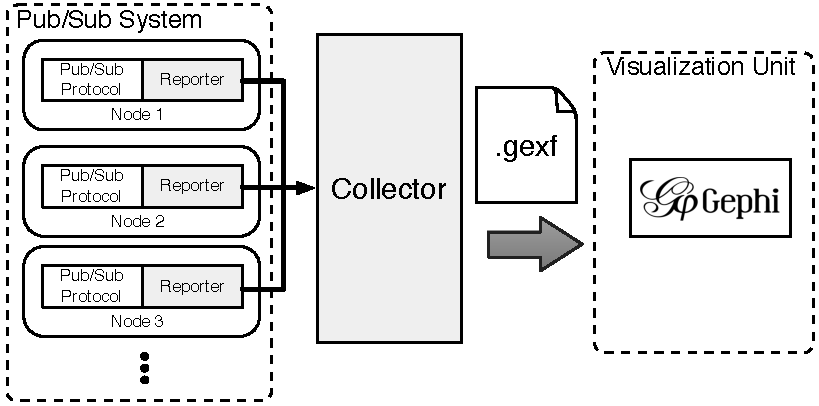
\includegraphics[width=\linewidth]{figures/arch}
\caption{Architecture diagram of \demo}
\label{fig:arch}
\end{figure}
\section{Examples of visualizations for PolderCast and Scribe}
\section{VizPub as a tool for evaluating pub/sub systems }
\subsection{Benefits to our approach}

\section{Using Test-Driven Development}

Software Development Methodology is an active area of research
which is in part driven by the business needs of the private
sector\cite{janzen2005test}. One popular practice is so-called Test-Driven
Development (TDD). The promoters of TDD claims it increases
productivity and reduces the number of bugs and defects in the
code significantly~\cite{beck2003test}. Research
efforts performed at IBM~\cite{maximilien2003assessing} seems to
lend credibility to these claims. However, the use of TDD is not
prevalent in academia, and in~\cite{janzen2005test} they
recommend further research into the field in order to better
determine its effects.

Using TDD means writing tests before writing any code. There are
different types of test. \emph{Unit Tests} targets small,
independent pieces of code, typically methods within a single
module or component, while \emph{Integration Tests} aim to test
code across such modules and components in order to determine
how well they integrate with each other. In our work, we only
took advantage of Unit Tests where suitable using the
JUnit~\cite{junit} and Mockito~\cite{mockito} libraries.
We could also have benefited from a suite of integration tests,
as our implementation is heavily dependent on interoperating
components, as well as file and network IO\@. However, writing
these sort of tests would simply be too time consuming compared
to writing smaller unit tests.

The TDD approach to software development is best described through the
Red-Green-Refactor mantra, which is a central part of the
TDD-philosophy. It can be described through the following steps:

\begin{description}
    \item[Step 1:] Write a test that fails. (Red)
    \item[Step 2:] Make the test pass. (Green)
    \item[Step 3:] Refactor the code while making sure the test
        still passes. (Refactor)
\end{description}

In our experience this routine has been helpful when working
with our implementation code, as it enables us as developer to
refactor with confidence achieving more maintainable code and a
more thoughtful software design. Since we share our
implementation code with the research community by hosting it in
a open repository, any tool or method that helps us improve the
design and maintainability of our project is of great value to
us. Using TDD forced us to think more deeply about what
functionality to implement and how to structure and split the
problem domain into smaller function points. We believe that in
the end, following TDD where its suitable is beneficial to both
programmer productivity as well as programmer happiness. Also,
we are confident that this practice decreased the amount of
technical debt in our project, a problem we find to be commonplace in academia.
